\documentclass[11pt,a4paper]{article}
\usepackage[utf8]{inputenc}
\usepackage[T1]{fontenc}
\usepackage{lmodern}
\usepackage[margin=2.4cm]{geometry}
\usepackage{amsmath,amssymb}
\usepackage{booktabs}
\usepackage{graphicx}
\usepackage{xcolor}
\usepackage{microtype}
\usepackage[colorlinks=true,linkcolor=blue!50!black,urlcolor=blue!50!black,citecolor=blue!50!black]{hyperref}

% generated by make_figures.py; do not edit
\newcommand{\SquareWorstRelDev}{6.2}
\newcommand{\SqThGaussHalf}{0.643}
\newcommand{\SqThGaussOne}{12.999}
\newcommand{\SqThGaussTwo}{76.546}
\newcommand{\SqThGaussFour}{365.789}
\newcommand{\SqThRieszThree}{1.584}
\newcommand{\SqThRieszFour}{4.210}
\newcommand{\SqThRieszSix}{12.500}
\newcommand{\LatGaussHalf}{1.008477919}
\newcommand{\LatGaussOne}{0.159595267}
\newcommand{\LatGaussTwo}{0.004238959299}
\newcommand{\LatGaussFour}{2.994792998e-06}
\newcommand{\LatRieszThree}{8.8927451}
\newcommand{\LatRieszFour}{5.7833593}
\newcommand{\LatRieszSix}{4.141256547}
\newcommand{\LatYukawaOne}{3.250642679}
\newcommand{\LatYukawaTwo}{0.7870856979}
\newcommand{\GapAYukawaOne}{2.2}
\newcommand{\GapAYukawaTwo}{5.5}
\newcommand{\GapBYukawaOne}{1.5}
\newcommand{\GapBYukawaTwo}{3.6}
\newcommand{\NA}{1619}
\newcommand{\SpacingA}{9.24}
\newcommand{\GapAGaussHalf}{4.2}
\newcommand{\GapAGaussOne}{26.0}
\newcommand{\GapARieszThree}{4.3}
\newcommand{\GapARieszFour}{10.6}
\newcommand{\GapARieszSix}{32.3}
\newcommand{\NB}{4225}
\newcommand{\SpacingB}{5.71}
\newcommand{\GapBGaussHalf}{3.0}
\newcommand{\GapBGaussOne}{16.0}
\newcommand{\GapBRieszThree}{2.7}
\newcommand{\GapBRieszFour}{6.5}
\newcommand{\GapBRieszSix}{18.7}


\newcommand{\repo}{\href{https://github.com/xaviercallens/triangular-universal-optimality-lean}{\texttt{triangular-universal-optimality-lean}}}
\newcommand{\code}[1]{\texttt{#1}}
\newcommand{\Rp}{\mathbb{R}^2}

\title{The triangular-lattice energy bound:\\a guide for physicists}
\author{Xavier Callens (SocrateAI Lab)\thanks{Prepared with Claude (Anthropic) AI agents under the author's direction.
All Lean results, numerics and figures are reproducible from the repository \repo; nothing here has been peer reviewed.}}
\date{Release v0.3.0, 11 October 2026}

\begin{document}
\maketitle

\noindent\fbox{\parbox{\dimexpr\linewidth-2\fboxsep-2\fboxrule}{\small
\textbf{Status.} The mathematics below is kernel-checked in Lean~4 \emph{conditional on} an AI-generated upstream
theorem (openai/math, \code{universal\_energy\_minimum}) whose Lean definitions no human has yet audited against the
Cohn--Kumar conjecture. Nothing here settles that conjecture. The physical case study is consistency evidence (Tier~X),
not a validation of the theorem. Open problems and how to help: \href{https://github.com/xaviercallens/triangular-universal-optimality-lean/blob/main/RED_TEAM.md}{\code{RED\_TEAM.md}}.}}

\section*{What you can use, in one paragraph}

For any homogeneous two-dimensional system of identical particles with a pair repulsion $V(r)=g(r^2)$, where $g$ is
\emph{completely monotone}, the energy per particle at density $\rho$ can never be lower than that of the triangular
lattice at the same density. This holds among \emph{all} configurations (not only lattices), and we give the
lattice value in closed form or as a fast series (Section~\ref{sec:values}). For data, the companion tool
\code{physics/ubound.py} tells you how far a measured or simulated configuration sits above that floor, with controls that
say whether the answer is resolved (Section~\ref{sec:tool}). We ran it on measured skyrmion lattices
(Section~\ref{sec:case}).

\section{The statement in physics language}\label{sec:statement}

\paragraph{Setting.} A configuration is a set $C\subset\Rp$ of particle positions with finitely many points in every
bounded region. Its density is $\rho=\lim_{R\to\infty} N_R/(\pi R^2)$, where $N_R$ counts particles within distance $R$
of the origin. For a pair potential $V(r)=g(r^2)$ the \emph{energy per particle} is
\begin{equation}
  E_g(C)=\liminf_{R\to\infty}\frac{1}{N_R}\sum_{x\in C\cap B_R}\;\sum_{y\in C\cap B_R,\,y\neq x} g\bigl(|x-y|^2\bigr).
  \label{eq:energy}
\end{equation}
Each pair is counted twice: the usual physical energy per particle is $\tfrac12E_g$. All comparisons below are
ratios, so the convention cancels.

\paragraph{The admissible class.} $g:(0,\infty)\to[0,\infty)$ is smooth and \emph{completely monotone}:
$(-1)^k g^{(k)}(t)\ge0$ for all $k$ and $t>0$. Equivalently (Bernstein), $g(t)=\int e^{-ut}\,d\mu(u)$ is a
superposition of Gaussians in the distance. Table~\ref{tab:class} lists common interactions.

\begin{table}[h]
\centering\small
\begin{tabular}{@{}lllp{6.1cm}@{}}
\toprule
Interaction & $V(r)$ & In the class? & Status here \\
\midrule
Gaussian core & $e^{-\pi\alpha r^2}$ & yes & Tier A: upstream's admissibility applies directly \\
Riesz / inverse power & $r^{-s}$ & yes & Tier A (D1). Informative for $s>2$; for $s\le2$ the lattice sum diverges \\
Dipolar colloids & $r^{-3}$ & yes ($s=3$) & Tier A, special case of Riesz \\
Yukawa / screened Coulomb & $e^{-\kappa r}/r$ & yes & Tier C: written argument (composition rule, CKMRV footnote~2), not kernel-checked \\
Thin-film vortices (Pearl) & $K_0(r/\lambda)$ & yes & Tier C: $K_0(\sqrt t)$ is a Gaussian mixture; not formalised \\
Coulomb, log gas & $1/r$, $-\log r$ & -- & not covered: needs renormalised (jellium) energies; upstream states this, not in Lean \\
Lennard-Jones, soft shoulders & -- & no & not covered: not completely monotone \\
\bottomrule
\end{tabular}
\caption{Which physical interactions the bound covers. Tier A = kernel-checked consequence of the upstream theorem;
Tier C = argument written out but not machine-checked.}\label{tab:class}
\end{table}

\paragraph{The theorem (D2).} For every admissible $g$, every $\rho>0$ and every configuration $C$ of density $\rho$,
\begin{equation}
  E_g(C)\;\ge\;E_g\bigl(\rho^{-1/2}A\bigr)=\sum_{a\in A\setminus 0} g\bigl(|a|^2/\rho\bigr),
  \label{eq:bound}
\end{equation}
where $A$ is the triangular lattice with one point per unit area, and the rescaled lattice $\rho^{-1/2}A$ attains the
bound. The Lean names are:
\begin{itemize}\setlength\itemsep{0pt}\small
\item D2, every density: \code{TriangularDensity.triangular\_optimal\_any\_density};
\item D1, Riesz: \code{TriangularRiesz.triangular\_riesz\_optimal};
\item D3, CKMRV's definition with lower energy:\\ \code{TriangularUniversalOptimality.triangular\_universally\_optimal}.
\end{itemize}

\paragraph{Three facts a physicist should not miss.}
\begin{enumerate}
\item \emph{The minimum value is pinned, not the minimiser.} Removing one particle from the lattice changes neither
the density nor the energy, so a lattice with a vacancy is also a minimiser (Lean:
\code{universal\_optimum\_not\_unique}; this is CKMRV's remark after their Theorem~1.4). The bound cannot by itself
predict that a system crystallises. It predicts that nothing can beat the crystal's energy.
\item \emph{The density must be fixed.} Comparing a configuration with the lattice at a different density is
meaningless, and the unrescaled statement is provably false (Lean: \code{unscaled\_false}). This is why the density
estimate dominates the numerics (Section~\ref{sec:tool}).
\item \emph{Boundary conventions do not matter.} Counting with open or closed disks gives the same density and energy
for every configuration (D4, \code{TriangularOpenDiskAny}). Other window shapes, $\limsup$ energies and physical
boundary conditions (walls, traps, neutralising backgrounds) are \emph{not} covered.
\end{enumerate}

\section{How sure is this?}\label{sec:status}

\begin{center}\small
\begin{tabular}{@{}p{5.2cm}p{9.2cm}@{}}
\toprule
Claim & Evidence \\
\midrule
Upstream proof is correct & Lean kernel accepts it with only \code{propext}, \code{Classical.choice}, \code{Quot.sound}.
The proof is AI-generated and not peer reviewed. \\
Upstream definitions mean Cohn--Kumar & Audited line by line against CKMRV by an AI agent only. \textbf{This is the main open
question.} Known gap: the lower energy ($\liminf$) replaces CKMRV's requirement that the energy limit exists. \\
Corollaries D1--D4 & 31 theorems kernel-checked; clean rebuild from source passes the axiom gate
(\code{verification/rebuild\_v0.2.0/}); planted \code{sorry} and fake-axiom controls are caught. \\
Lattice values (Section~\ref{sec:values}) & Closed forms reproduced to 10 digits and cross-checked by direct sums. \\
Status of the conjecture & The latest paper we found (arXiv:2511.03353, Nov.\ 2025) proves \emph{local} optimality and calls
global optimality open; we found no published assessment of the upstream claim. \\
\bottomrule
\end{tabular}
\end{center}

\section{The floor, in numbers}\label{sec:values}

At density $\rho$ the lattice energy is $E_g(\rho)=\sum_{a\in A\setminus0} g(|a|^2/\rho)$, with
$|a|^2=\tfrac{2}{\sqrt3}(j^2+jk+k^2)$ for $a=a(j,k)$. Two families have closed forms.

\paragraph{Riesz.} With $\sigma=s/2$ and $L(\sigma,\chi_{-3})=3^{-\sigma}\bigl(\zeta(\sigma,\tfrac13)-\zeta(\sigma,\tfrac23)\bigr)$,
\begin{equation}
  E_{r^{-s}}(\rho)=\rho^{s/2}\Bigl(\tfrac{2}{\sqrt3}\Bigr)^{-s/2}\,6\,\zeta(\tfrac s2)\,L(\tfrac s2,\chi_{-3}),\qquad s>2.
\end{equation}
The $\rho^{s/2}$ scaling is itself kernel-checked (\code{riesz\_lattice\_homogeneous}). For the square lattice,
$6\zeta L$ becomes $4\zeta(\sigma)\beta(\sigma)$ and the prefactor $(2/\sqrt3)^{-\sigma}$ disappears.

\paragraph{Gaussian.} $E(\rho)=\theta_A(\alpha/\rho)-1$ with $\theta_A(\alpha)=\sum_{a\in A}e^{-\pi\alpha|a|^2}$; the
series converges in a handful of shells. For the square lattice it is $\theta_3(e^{-\pi\alpha})^2-1$.

\begin{table}[h]
\centering\small
\begin{tabular}{@{}lrrl@{}}
\toprule
$V(r)$, density 1 & triangular floor & square excess & source \\
\midrule
$e^{-\pi r^2/2}$ & \LatGaussHalf & \SqThGaussHalf\,\% & theta series \\
$e^{-\pi r^2}$ & \LatGaussOne & \SqThGaussOne\,\% & theta series \\
$e^{-2\pi r^2}$ & \LatGaussTwo & \SqThGaussTwo\,\% & theta series \\
$r^{-3}$ & \LatRieszThree & \SqThRieszThree\,\% & Epstein zeta, closed form \\
$r^{-4}$ & \LatRieszFour & \SqThRieszFour\,\% & Epstein zeta, closed form \\
$r^{-6}$ & \LatRieszSix & \SqThRieszSix\,\% & Epstein zeta, closed form \\
$e^{-r}/r$ (Tier C) & \LatYukawaOne & -- & direct sum \\
$e^{-2r}/r$ (Tier C) & \LatYukawaTwo & -- & direct sum \\
\bottomrule
\end{tabular}
\caption{Energy per particle (ordered pairs, eq.~\ref{eq:energy}) of the triangular lattice at density 1, and how much
higher the square lattice sits. At density $\rho$, rescale lengths by $\rho^{-1/2}$ (Riesz: multiply by $\rho^{s/2}$).
Generated from \code{physics/results/}; no value is typed by hand.}\label{tab:values}
\end{table}

\section{Testing the bound on your own data}\label{sec:tool}

\paragraph{The estimator.} Rescale positions to density 1, keep the \emph{inner} particles (farther than $R_c=6$ mean
spacings from the window edge, so their neighbourhoods are complete), and average their energies, summing neighbours
within $R_c$. For Riesz potentials, add the uniform tail $2\pi R_c^{2-s}/(s-2)$; for Yukawa, add
$2\pi e^{-\kappa R_c}/\kappa$. The relative gap $(E_\text{data}-E_\text{lattice})/E_\text{lattice}$ is the result.

\paragraph{The numerical improvement: density from Voronoi cells.} Everything hinges on $\rho$, because the comparison
is at fixed density. Our first preregistered runs (P1, P1b) estimated $\rho$ by counting particles in a box, and the
boundary made even a perfect lattice look 3--10\,\% off, more than the square-vs-triangle difference for soft
potentials. Estimating $\rho$ from the Voronoi cells of the \emph{same} inner particles whose energies are averaged gives
each cell of a perfect lattice an area of exactly $1/\rho$. The calibration error fell by up to twelve orders of
magnitude (Figure~\ref{fig:cal}); what remains for Riesz is the tail approximation.

\begin{figure}[h]
\centering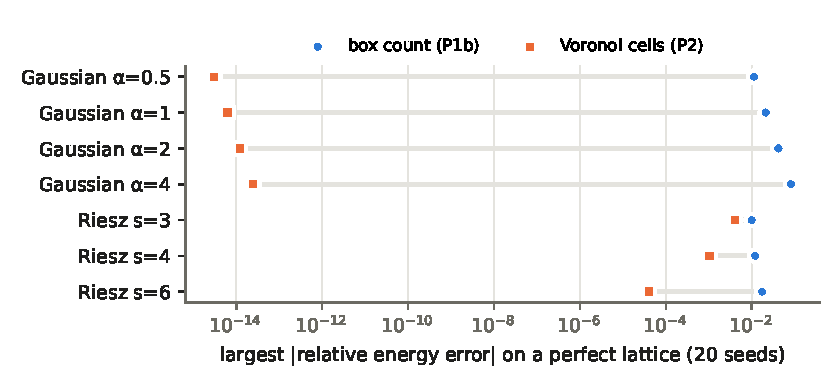
\includegraphics[width=0.82\linewidth]{fig_calibration.pdf}
\caption{Largest relative energy error that the estimator assigns to a \emph{perfect} triangular lattice (20 random
placements, same size as the 338\,K snapshot). Box counting (P1b) versus Voronoi cells (P2).}\label{fig:cal}
\end{figure}

\paragraph{The controls the tool runs for you.} Every potential gets a verdict only if the estimator can resolve it on
synthetic data of the same size and shape:
C1 perfect lattices calibrate a tolerance (three times the worst error);
C2 jittered lattices must sit above it and rise with the jitter;
C3 a square lattice must sit above it;
C4 comparing the data with the lattice at the wrong density (1.3$\rho$) must be able to violate the bound, which shows
the test can fail. Figure~\ref{fig:theory} shows that C3 reproduces the exact square-lattice excess of
Table~\ref{tab:values}; the worst deviation is \SquareWorstRelDev\,\%, from the Riesz $s=3$ tail.

\begin{figure}[h]
\centering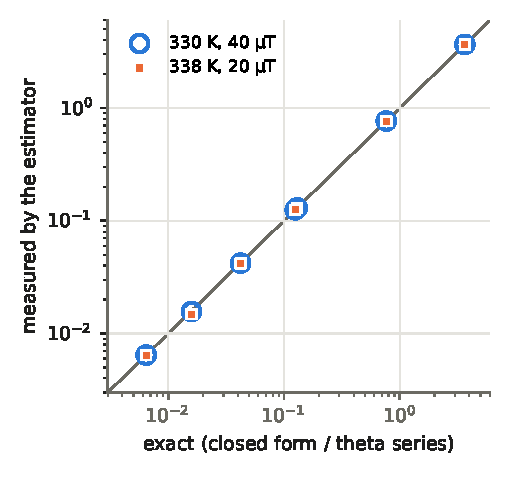
\includegraphics[width=0.46\linewidth]{fig_theory.pdf}
\caption{Square-lattice excess over the triangular floor: measured by the estimator (control C3) versus the exact value
(closed forms and theta series), for all seven potentials and both snapshot geometries.}\label{fig:theory}
\end{figure}

\paragraph{Running it.}
\begin{verbatim}
python3 physics/ubound.py --self-test
python3 physics/ubound.py positions.csv --cols 0,1 \
        --potentials gauss:1,riesz:3,riesz:6,yukawa:1 --json result.json
\end{verbatim}
Units do not matter (only ratios do). Verdicts are \emph{above the bound (resolved)}, \emph{at the bound within
tolerance}, \emph{unresolved} (the controls failed, so the number means nothing) or \emph{below the bound}
(exit code 1: check your data before anything else).

\paragraph{When not to use it.} The bound is about homogeneous bulk density. Particles in a trap, near a wall or with a
density gradient are outside it. Mixtures, polydisperse particles and attractive or non-monotone interactions are
outside it. With fewer than about a thousand particles, few potentials will resolve. For Riesz $s\le2$ (Coulomb, log) the
floor is infinite and the test is vacuous.

\section{Case study: measured skyrmion lattices}\label{sec:case}

\paragraph{Data.} Kerr-microscopy positions of skyrmions in a magnetic thin-film multilayer, two snapshots:
\NA\ skyrmions at 330\,K, 40\,$\mu$T (mean spacing \SpacingA\,$\mu$m) and \NB\ at 338\,K, 20\,$\mu$T
(\SpacingB\,$\mu$m). Zenodo \href{https://doi.org/10.5281/zenodo.4450305}{doi:10.5281/zenodo.4450305} (CC-BY-4.0),
from the article arXiv:2004.09244; all credit for the measurements to its authors. The tool downloads the archive and
checks its md5 against Zenodo.

\paragraph{Why skyrmions are a legitimate input.} Inequality~\eqref{eq:bound} holds for \emph{every} configuration and
\emph{every} admissible $g$, whatever the particles' real interaction. Any measured pattern is therefore a valid test
input. Short Gaussians probe the nearest-neighbour structure, Riesz potentials probe longer range.

\paragraph{Result (P2, preregistered, gate PASS).} Both snapshots sit above the floor for every potential, and every
gap exceeds its tolerance (Figure~\ref{fig:data}):
\begin{center}\small
\begin{tabular}{@{}lrrrrrrr@{}}
\toprule
 & $e^{-\pi r^2/2}$ & $e^{-\pi r^2}$ & $r^{-3}$ & $r^{-4}$ & $r^{-6}$ & $e^{-r}/r$ & $e^{-2r}/r$ \\
\midrule
330\,K & +\GapAGaussHalf\,\% & +\GapAGaussOne\,\% & +\GapARieszThree\,\% & +\GapARieszFour\,\% & +\GapARieszSix\,\% & +\GapAYukawaOne\,\% & +\GapAYukawaTwo\,\% \\
338\,K & +\GapBGaussHalf\,\% & +\GapBGaussOne\,\% & +\GapBRieszThree\,\% & +\GapBRieszFour\,\% & +\GapBRieszSix\,\% & +\GapBYukawaOne\,\% & +\GapBYukawaTwo\,\% \\
\bottomrule
\end{tabular}
\end{center}
The Yukawa columns are Tier C and come from \code{ubound.py} (for $e^{-r/2}/r$ the tool reports \emph{unresolved}).
The colder, higher-field snapshot sits further above the floor for every potential.

\begin{figure}[h]
\centering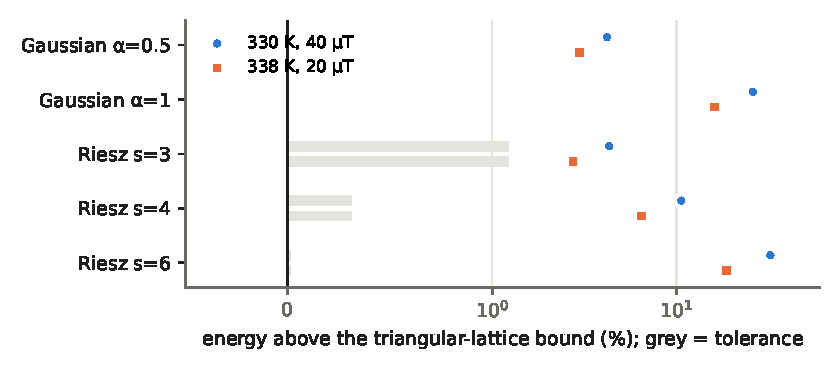
\includegraphics[width=0.82\linewidth]{fig_data.pdf}
\caption{Energy of the measured skyrmion configurations above the triangular-lattice floor at the same density (P2).
Grey bars: tolerance from the perfect-lattice control (invisible for Gaussians, about $10^{-14}$). Symmetric-log axis.}\label{fig:data}
\end{figure}

\paragraph{What this does and does not show.} No measured configuration beats the floor, and the gaps are resolved,
which is what the theorem's physical reading predicts. But both snapshots are perturbed triangular lattices, and
results that were already known (lattice-only optimality; local optimality, arXiv:2511.03353) predict the same sign. So
this case cannot tell the new global statement apart from them. The process record matters: the first preregistered
run (P1) and its amendment (P1b) \emph{failed} their own sensitivity checks with box counting. They are kept unchanged in
the repository, and P2 was preregistered before it ran, but its data verdict was not blind.

\section{Where a physicist can help}

\begin{itemize}
\item \textbf{Read the upstream definitions} (density, energy, admissible potential) against CKMRV, Section~1. This is
the main open question, and it needs no Lean (target T1).
\item \textbf{Bring data from a disordered or non-lattice system}, such as a 2D glass, a quenched colloidal liquid or a
hexatic phase. There, known results do not already predict the sign, so the comparison means more.
\item \textbf{Systems with a known completely monotone interaction} (dipolar colloids, $r^{-3}$; dusty plasma, Yukawa)
would give the gap a direct energetic meaning.
\end{itemize}

\section*{References}
\small
\begin{itemize}\setlength\itemsep{0pt}
\item H.~Cohn, A.~Kumar, \emph{Universally optimal distribution of points on spheres}, J.~Amer.\ Math.\ Soc.\ 20 (2007).
\item H.~Cohn, A.~Kumar, S.~D.~Miller, D.~Radchenko, M.~Viazovska, \emph{Universal optimality of the $E_8$ and Leech
lattices and interpolation formulas}, Ann.\ of Math.\ 196 (2022), arXiv:1902.05438.
\item H.~L.~Montgomery, \emph{Minimal theta functions}, Glasgow Math.\ J.\ 30 (1988).
\item \emph{The hexagonal lattice is universally locally optimal}, arXiv:2511.03353 (2025).
\item openai/math, \emph{Universal optimality of the triangular lattice} (manuscript, 2026-09-23) and Lean development,
\url{https://github.com/openai/math}.
\item Skyrmion data: Zenodo doi:10.5281/zenodo.4450305; article arXiv:2004.09244.
\item This work: doi:10.5281/zenodo.23285631 (D1--D2), doi:10.5281/zenodo.23293429 (D3); repository \repo.
\end{itemize}

\end{document}
